\chapter{Cluster distortion and bipolaron formation}
\label{chap:ground}

We performed a series of diagonalizations of the hamiltonian matrix (\ref{eq:full-hamiltonian}) using the parameters described in section \ref{sec:model-parameters} with a variable infrared charge-lattice coupling, $\lambda_{ir}$. 
We took $\lambda_{ir}$ values in the representative range from 0 eV to 0.25 eV. 
This range allowed us to explore the behaviour of the system in the small, middle and strong coupling regimes. 
Besides the eigenvalues and eigenvectors of the hamiltonian we also calculated the mean phonon number with their dispersions and the projections into phonon coordinates $(u_{ir}, u_R)$ (see section \ref{sec:lattice-distortions}).

In this chapter we turn our attention to the ground and first excited states of the system since only the first excitation in the (\ref{eq:full-hamiltonian}) hamiltonian has a sufficiently low energy to be significantly occuppied in the temperature range where the pseudogap phase is present.
All other excitations have an energy above $T=\omega_i/k_B \sim 550$ K (see Figure \ref{fig:irSpectra}).
First we calculate the difference in Cu-O bond lengths (if any) as a function of the $\lambda_{ir}$ coupling parameter.
With this we can find the $\lambda_{ir}$ value that reproduces the 0.13 \AA\ observed cluster distortion \cite{MustredeLeon1990}.
From the projection into phonon coordinates we can observe whether this distortion is static or dynamic for different $\lambda_{ir}$ values \cite{MustredeLeon1992}.
The presence of a dynamic cluster distortion signals a correlated movement between atomic centers and charged particles, that is, it signals polaronic behaviour.
The difference between the ground state energy in the absence of charge-lattice interaction ($\lambda_{ir}=0$) and its value for the coupling value where this polaronic behaviour sets can be identified as the \textit{bipolaron binding energy}.
We estimate this binding energy for the experimentally relevant $\lambda_{ir}$ value and compare it to other calculations.
Finally we model an isotopic oxygen substitution $^{16}$O$\rightarrow ^{18}$O and calculate its effects in the bipolaron binding energy.

\section{Cu(1)-O(4) local distortion}
\label{sec:grd-phonon-proj}

The wavefunction projection into phonon coordinates (\ref{eq:phonon-coord-projection}) gives information about the coodinates of the three atoms in the CuO$_2$ cluster.
In particular, the infrared phonon coordinate $u_{ir}$ is directly proportional to the bond distortion in the CuO$_2$ cluster, $d$, as shown in (\ref{eq:dvsuir}).
Since the ground state has zero Raman phonons and we have set $\lambda_R=0$, its projection into $u_R$ will remain unchanged and given by a simple gaussian distribution.
Thus, setting $u_R=0$, we projected the ground state into $u_{ir}$ for different $\lambda_{ir}$ values.
In the left panel of Figure \ref{fig:uirCoupl} we show a plot of these projections.
The projection has a gaussian shape for $\lambda_{ir}=0$.
However, as $\lambda_{ir}$ increases it smoothly develops into two separated peaks.
For a small range in the middle coupling values there are clearly two peaks but they are not separated. 
Since the system will tend to be near the maximum values of this projections this results can be interpreted as follows: in the small coupling range the bond distances remain equal albeit with an increased uncertainty; in the middle coupling range two Cu-O distances develop but the system can \textit{tunnel} between them, that is, the distortion is \textit{dynamic}; finally in the strong coupling range the two peaks are fully separated and the distortion becomes \textit{static}.
Only in the small range $\sim 0.12 - 0.16$ eV the bond distortion has set in and it is dynamical in nature.
%
\begin{figure}[ht]
  \centering
  % GNUPLOT: LaTeX picture with Postscript
\begingroup
  \makeatletter
  \providecommand\color[2][]{%
    \GenericError{(gnuplot) \space\space\space\@spaces}{%
      Package color not loaded in conjunction with
      terminal option `colourtext'%
    }{See the gnuplot documentation for explanation.%
    }{Either use 'blacktext' in gnuplot or load the package
      color.sty in LaTeX.}%
    \renewcommand\color[2][]{}%
  }%
  \providecommand\includegraphics[2][]{%
    \GenericError{(gnuplot) \space\space\space\@spaces}{%
      Package graphicx or graphics not loaded%
    }{See the gnuplot documentation for explanation.%
    }{The gnuplot epslatex terminal needs graphicx.sty or graphics.sty.}%
    \renewcommand\includegraphics[2][]{}%
  }%
  \providecommand\rotatebox[2]{#2}%
  \@ifundefined{ifGPcolor}{%
    \newif\ifGPcolor
    \GPcolortrue
  }{}%
  \@ifundefined{ifGPblacktext}{%
    \newif\ifGPblacktext
    \GPblacktextfalse
  }{}%
  % define a \g@addto@macro without @ in the name:
  \let\gplgaddtomacro\g@addto@macro
  % define empty templates for all commands taking text:
  \gdef\gplbacktext{}%
  \gdef\gplfronttext{}%
  \makeatother
  \ifGPblacktext
    % no textcolor at all
    \def\colorrgb#1{}%
    \def\colorgray#1{}%
  \else
    % gray or color?
    \ifGPcolor
      \def\colorrgb#1{\color[rgb]{#1}}%
      \def\colorgray#1{\color[gray]{#1}}%
      \expandafter\def\csname LTw\endcsname{\color{white}}%
      \expandafter\def\csname LTb\endcsname{\color{black}}%
      \expandafter\def\csname LTa\endcsname{\color{black}}%
      \expandafter\def\csname LT0\endcsname{\color[rgb]{1,0,0}}%
      \expandafter\def\csname LT1\endcsname{\color[rgb]{0,1,0}}%
      \expandafter\def\csname LT2\endcsname{\color[rgb]{0,0,1}}%
      \expandafter\def\csname LT3\endcsname{\color[rgb]{1,0,1}}%
      \expandafter\def\csname LT4\endcsname{\color[rgb]{0,1,1}}%
      \expandafter\def\csname LT5\endcsname{\color[rgb]{1,1,0}}%
      \expandafter\def\csname LT6\endcsname{\color[rgb]{0,0,0}}%
      \expandafter\def\csname LT7\endcsname{\color[rgb]{1,0.3,0}}%
      \expandafter\def\csname LT8\endcsname{\color[rgb]{0.5,0.5,0.5}}%
    \else
      % gray
      \def\colorrgb#1{\color{black}}%
      \def\colorgray#1{\color[gray]{#1}}%
      \expandafter\def\csname LTw\endcsname{\color{white}}%
      \expandafter\def\csname LTb\endcsname{\color{black}}%
      \expandafter\def\csname LTa\endcsname{\color{black}}%
      \expandafter\def\csname LT0\endcsname{\color{black}}%
      \expandafter\def\csname LT1\endcsname{\color{black}}%
      \expandafter\def\csname LT2\endcsname{\color{black}}%
      \expandafter\def\csname LT3\endcsname{\color{black}}%
      \expandafter\def\csname LT4\endcsname{\color{black}}%
      \expandafter\def\csname LT5\endcsname{\color{black}}%
      \expandafter\def\csname LT6\endcsname{\color{black}}%
      \expandafter\def\csname LT7\endcsname{\color{black}}%
      \expandafter\def\csname LT8\endcsname{\color{black}}%
    \fi
  \fi
  \setlength{\unitlength}{0.0500bp}%
  \begin{picture}(8502.00,3968.00)%
    \gplgaddtomacro\gplbacktext{%
      \colorrgb{0.31,0.31,0.31}%
      \put(990,595){\makebox(0,0)[r]{\strut{}\scriptsize 0}}%
      \colorrgb{0.31,0.31,0.31}%
      \put(990,844){\makebox(0,0)[r]{\strut{}\scriptsize 0.02}}%
      \colorrgb{0.31,0.31,0.31}%
      \put(990,1092){\makebox(0,0)[r]{\strut{}\scriptsize 0.04}}%
      \colorrgb{0.31,0.31,0.31}%
      \put(990,1341){\makebox(0,0)[r]{\strut{}\scriptsize 0.06}}%
      \colorrgb{0.31,0.31,0.31}%
      \put(990,1590){\makebox(0,0)[r]{\strut{}\scriptsize 0.08}}%
      \colorrgb{0.31,0.31,0.31}%
      \put(990,1838){\makebox(0,0)[r]{\strut{}\scriptsize 0.1}}%
      \colorrgb{0.31,0.31,0.31}%
      \put(990,2087){\makebox(0,0)[r]{\strut{}\scriptsize 0.12}}%
      \colorrgb{0.31,0.31,0.31}%
      \put(990,2335){\makebox(0,0)[r]{\strut{}\scriptsize 0.14}}%
      \colorrgb{0.31,0.31,0.31}%
      \put(990,2584){\makebox(0,0)[r]{\strut{}\scriptsize 0.16}}%
      \colorrgb{0.31,0.31,0.31}%
      \put(990,2833){\makebox(0,0)[r]{\strut{}\scriptsize 0.18}}%
      \colorrgb{0.31,0.31,0.31}%
      \put(990,3081){\makebox(0,0)[r]{\strut{}\scriptsize 0.2}}%
      \colorrgb{0.31,0.31,0.31}%
      \put(990,3330){\makebox(0,0)[r]{\strut{}\scriptsize 0.22}}%
      \colorrgb{0.31,0.31,0.31}%
      \put(990,3579){\makebox(0,0)[r]{\strut{}\scriptsize 0.24}}%
      \colorrgb{0.31,0.31,0.31}%
      \put(1267,328){\makebox(0,0){\strut{}\scriptsize -0.4}}%
      \colorrgb{0.31,0.31,0.31}%
      \put(1889,328){\makebox(0,0){\strut{}\scriptsize -0.2}}%
      \colorrgb{0.31,0.31,0.31}%
      \put(2512,328){\makebox(0,0){\strut{}\scriptsize 0}}%
      \colorrgb{0.31,0.31,0.31}%
      \put(3134,328){\makebox(0,0){\strut{}\scriptsize 0.2}}%
      \colorrgb{0.31,0.31,0.31}%
      \put(3756,328){\makebox(0,0){\strut{}\scriptsize 0.4}}%
      \csname LTb\endcsname%
      \put(484,2149){\rotatebox{-270}{\makebox(0,0){\strut{}$\lambda_{ir}$ (eV)}}}%
      \put(2511,-2){\makebox(0,0){\strut{}$u_{ir}$ (\AA)}}%
    }%
    \gplgaddtomacro\gplfronttext{%
    }%
    \gplgaddtomacro\gplbacktext{%
      \colorrgb{0.31,0.31,0.31}%
      \put(5241,595){\makebox(0,0)[r]{\strut{}\scriptsize 0}}%
      \colorrgb{0.31,0.31,0.31}%
      \put(5241,844){\makebox(0,0)[r]{\strut{}\scriptsize 0.02}}%
      \colorrgb{0.31,0.31,0.31}%
      \put(5241,1092){\makebox(0,0)[r]{\strut{}\scriptsize 0.04}}%
      \colorrgb{0.31,0.31,0.31}%
      \put(5241,1341){\makebox(0,0)[r]{\strut{}\scriptsize 0.06}}%
      \colorrgb{0.31,0.31,0.31}%
      \put(5241,1590){\makebox(0,0)[r]{\strut{}\scriptsize 0.08}}%
      \colorrgb{0.31,0.31,0.31}%
      \put(5241,1838){\makebox(0,0)[r]{\strut{}\scriptsize 0.1}}%
      \colorrgb{0.31,0.31,0.31}%
      \put(5241,2087){\makebox(0,0)[r]{\strut{}\scriptsize 0.12}}%
      \colorrgb{0.31,0.31,0.31}%
      \put(5241,2335){\makebox(0,0)[r]{\strut{}\scriptsize 0.14}}%
      \colorrgb{0.31,0.31,0.31}%
      \put(5241,2584){\makebox(0,0)[r]{\strut{}\scriptsize 0.16}}%
      \colorrgb{0.31,0.31,0.31}%
      \put(5241,2833){\makebox(0,0)[r]{\strut{}\scriptsize 0.18}}%
      \colorrgb{0.31,0.31,0.31}%
      \put(5241,3081){\makebox(0,0)[r]{\strut{}\scriptsize 0.2}}%
      \colorrgb{0.31,0.31,0.31}%
      \put(5241,3330){\makebox(0,0)[r]{\strut{}\scriptsize 0.22}}%
      \colorrgb{0.31,0.31,0.31}%
      \put(5241,3579){\makebox(0,0)[r]{\strut{}\scriptsize 0.24}}%
      \colorrgb{0.31,0.31,0.31}%
      \put(5420,328){\makebox(0,0){\strut{}\scriptsize -0.8}}%
      \colorrgb{0.31,0.31,0.31}%
      \put(5756,328){\makebox(0,0){\strut{}\scriptsize -0.6}}%
      \colorrgb{0.31,0.31,0.31}%
      \put(6091,328){\makebox(0,0){\strut{}\scriptsize -0.4}}%
      \colorrgb{0.31,0.31,0.31}%
      \put(6427,328){\makebox(0,0){\strut{}\scriptsize -0.2}}%
      \colorrgb{0.31,0.31,0.31}%
      \put(6763,328){\makebox(0,0){\strut{}\scriptsize 0}}%
      \colorrgb{0.31,0.31,0.31}%
      \put(7098,328){\makebox(0,0){\strut{}\scriptsize 0.2}}%
      \colorrgb{0.31,0.31,0.31}%
      \put(7434,328){\makebox(0,0){\strut{}\scriptsize 0.4}}%
      \colorrgb{0.31,0.31,0.31}%
      \put(7769,328){\makebox(0,0){\strut{}\scriptsize 0.6}}%
      \colorrgb{0.31,0.31,0.31}%
      \put(8105,328){\makebox(0,0){\strut{}\scriptsize 0.8}}%
      \csname LTb\endcsname%
      \put(4735,2149){\rotatebox{-270}{\makebox(0,0){\strut{}$\lambda_{ir}$ (eV)}}}%
      \put(6762,-2){\makebox(0,0){\strut{}$d$ (\AA)}}%
    }%
    \gplgaddtomacro\gplfronttext{%
    }%
    \gplbacktext
    \put(0,0){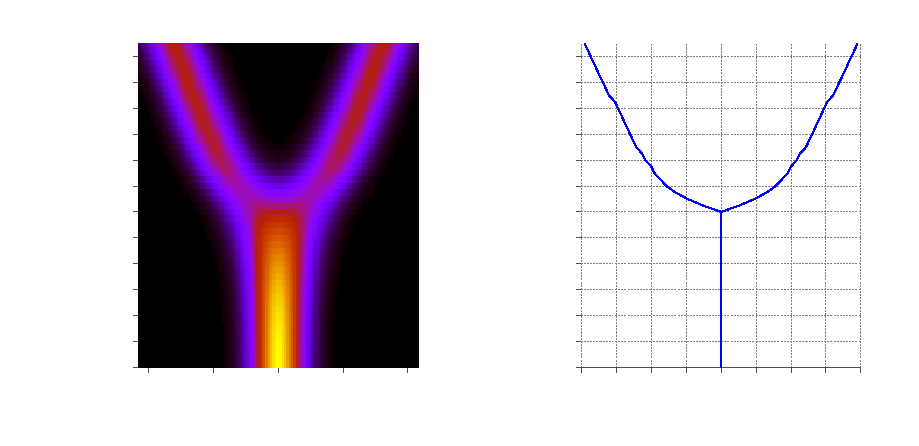
\includegraphics{images/uirCoupl}}%
    \gplfronttext
  \end{picture}%
\endgroup

  \caption{Projection into phonon coordinates (left panel) and calculated cluster distortion $d$ (right panel) for different $\lambda_{ir}$ coupling values with $u_R=0$.}
  \label{fig:uirCoupl}
\end{figure}

In the right panel of figure \ref{fig:uirCoupl} we show the cluster distortion $d$ assuming the system is found in a maximum value of the projection into phonon coordinates.
We observe that the distortion only sets in for $\lambda_{ir} > \sim 0.12$ eV and monotonically increases with $\lambda_{ir}$.
The two branches in this plot represent the two possible cluster distortions with the longer distance being in either of the CuO bonds.
The measured cluster distortion of $\sim 0.13$ \AA\ \cite{MustredeLeon1990} is reproduced in the intermedite coupling values. 
In particular, $\lambda_{ir}=0.1263$ eV reproduces that distortion.

The first excitation is an (antisymmetric) infrared-active state with one infrared phonon.
Contrary to the ground state, the antisymmetry of this excitation implies that it is zero at $u_{ir}=0$ for all $\lambda_{ir}$.
Also, the calculations show that increasing $\lambda_{ir}$ reduces the energy of this excitation asymptotically to zero (see Figure \ref{fig:irSpectra}) increasing its natural length scale. 
In Figure \ref{fig:phononProjGrdPol} we show the ground and first excited states projected into phonon coordinates $(u_R,u_{ir})$ for $\lambda_{ir}$ values in the weak, middle and strong coupling regimes.
The projection along $u_R$, as previously stated, is a simple gaussian in all cases.
In the middle coupling regime, with $\lambda_{ir}=0.1263$ eV, there are clearly two peaks present although, for the ground state, they are not fully separated.
For large coupling values the two peaks are fully separated in both states (static distortion) and the projections become very similar.

\begin{figure}[ht]
  \centering
  % GNUPLOT: LaTeX picture with Postscript
\begingroup
  \makeatletter
  \providecommand\color[2][]{%
    \GenericError{(gnuplot) \space\space\space\@spaces}{%
      Package color not loaded in conjunction with
      terminal option `colourtext'%
    }{See the gnuplot documentation for explanation.%
    }{Either use 'blacktext' in gnuplot or load the package
      color.sty in LaTeX.}%
    \renewcommand\color[2][]{}%
  }%
  \providecommand\includegraphics[2][]{%
    \GenericError{(gnuplot) \space\space\space\@spaces}{%
      Package graphicx or graphics not loaded%
    }{See the gnuplot documentation for explanation.%
    }{The gnuplot epslatex terminal needs graphicx.sty or graphics.sty.}%
    \renewcommand\includegraphics[2][]{}%
  }%
  \providecommand\rotatebox[2]{#2}%
  \@ifundefined{ifGPcolor}{%
    \newif\ifGPcolor
    \GPcolortrue
  }{}%
  \@ifundefined{ifGPblacktext}{%
    \newif\ifGPblacktext
    \GPblacktextfalse
  }{}%
  % define a \g@addto@macro without @ in the name:
  \let\gplgaddtomacro\g@addto@macro
  % define empty templates for all commands taking text:
  \gdef\gplbacktext{}%
  \gdef\gplfronttext{}%
  \makeatother
  \ifGPblacktext
    % no textcolor at all
    \def\colorrgb#1{}%
    \def\colorgray#1{}%
  \else
    % gray or color?
    \ifGPcolor
      \def\colorrgb#1{\color[rgb]{#1}}%
      \def\colorgray#1{\color[gray]{#1}}%
      \expandafter\def\csname LTw\endcsname{\color{white}}%
      \expandafter\def\csname LTb\endcsname{\color{black}}%
      \expandafter\def\csname LTa\endcsname{\color{black}}%
      \expandafter\def\csname LT0\endcsname{\color[rgb]{1,0,0}}%
      \expandafter\def\csname LT1\endcsname{\color[rgb]{0,1,0}}%
      \expandafter\def\csname LT2\endcsname{\color[rgb]{0,0,1}}%
      \expandafter\def\csname LT3\endcsname{\color[rgb]{1,0,1}}%
      \expandafter\def\csname LT4\endcsname{\color[rgb]{0,1,1}}%
      \expandafter\def\csname LT5\endcsname{\color[rgb]{1,1,0}}%
      \expandafter\def\csname LT6\endcsname{\color[rgb]{0,0,0}}%
      \expandafter\def\csname LT7\endcsname{\color[rgb]{1,0.3,0}}%
      \expandafter\def\csname LT8\endcsname{\color[rgb]{0.5,0.5,0.5}}%
    \else
      % gray
      \def\colorrgb#1{\color{black}}%
      \def\colorgray#1{\color[gray]{#1}}%
      \expandafter\def\csname LTw\endcsname{\color{white}}%
      \expandafter\def\csname LTb\endcsname{\color{black}}%
      \expandafter\def\csname LTa\endcsname{\color{black}}%
      \expandafter\def\csname LT0\endcsname{\color{black}}%
      \expandafter\def\csname LT1\endcsname{\color{black}}%
      \expandafter\def\csname LT2\endcsname{\color{black}}%
      \expandafter\def\csname LT3\endcsname{\color{black}}%
      \expandafter\def\csname LT4\endcsname{\color{black}}%
      \expandafter\def\csname LT5\endcsname{\color{black}}%
      \expandafter\def\csname LT6\endcsname{\color{black}}%
      \expandafter\def\csname LT7\endcsname{\color{black}}%
      \expandafter\def\csname LT8\endcsname{\color{black}}%
    \fi
  \fi
  \setlength{\unitlength}{0.0500bp}%
  \begin{picture}(7936.00,4534.00)%
    \gplgaddtomacro\gplbacktext{%
      \csname LTb\endcsname%
      \put(-63,2574){\makebox(0,0)[r]{\strut{}\scriptsize -0.3}}%
      \put(-63,2794){\makebox(0,0)[r]{\strut{}\scriptsize -0.2}}%
      \put(-63,3015){\makebox(0,0)[r]{\strut{}\scriptsize -0.1}}%
      \put(-63,3235){\makebox(0,0)[r]{\strut{}\scriptsize 0}}%
      \put(-63,3455){\makebox(0,0)[r]{\strut{}\scriptsize 0.1}}%
      \put(-63,3676){\makebox(0,0)[r]{\strut{}\scriptsize 0.2}}%
      \put(-63,3896){\makebox(0,0)[r]{\strut{}\scriptsize 0.3}}%
      \put(223,2094){\makebox(0,0){\strut{}\scriptsize -0.4}}%
      \put(799,2094){\makebox(0,0){\strut{}\scriptsize -0.2}}%
      \put(1375,2094){\makebox(0,0){\strut{}\scriptsize 0}}%
      \put(1951,2094){\makebox(0,0){\strut{}\scriptsize 0.2}}%
      \put(2527,2094){\makebox(0,0){\strut{}\scriptsize 0.4}}%
      \put(-569,3235){\rotatebox{-270}{\makebox(0,0){\strut{}$u_{R}$ (\AA)}}}%
      \put(1375,1808){\makebox(0,0){\strut{}}}%
      \put(794,4352){\makebox(0,0)[l]{\strut{}\scriptsize{$\lambda_{ir} = 0.00$ eV}}}%
    }%
    \gplgaddtomacro\gplfronttext{%
    }%
    \gplgaddtomacro\gplbacktext{%
      \csname LTb\endcsname%
      \put(2841,2094){\makebox(0,0){\strut{}\scriptsize -0.4}}%
      \put(3417,2094){\makebox(0,0){\strut{}\scriptsize -0.2}}%
      \put(3994,2094){\makebox(0,0){\strut{}\scriptsize 0}}%
      \put(4570,2094){\makebox(0,0){\strut{}\scriptsize 0.2}}%
      \put(5146,2094){\makebox(0,0){\strut{}\scriptsize 0.4}}%
      \put(3278,3235){\rotatebox{-270}{\makebox(0,0){\strut{}}}}%
      \put(3993,1808){\makebox(0,0){\strut{}}}%
      \put(3412,4352){\makebox(0,0)[l]{\strut{}\scriptsize{$\lambda_{ir} = 0.1263$ eV}}}%
    }%
    \gplgaddtomacro\gplfronttext{%
    }%
    \gplgaddtomacro\gplbacktext{%
      \csname LTb\endcsname%
      \put(5460,2094){\makebox(0,0){\strut{}\scriptsize -0.4}}%
      \put(6036,2094){\makebox(0,0){\strut{}\scriptsize -0.2}}%
      \put(6612,2094){\makebox(0,0){\strut{}\scriptsize 0}}%
      \put(7188,2094){\makebox(0,0){\strut{}\scriptsize 0.2}}%
      \put(7764,2094){\makebox(0,0){\strut{}\scriptsize 0.4}}%
      \put(5897,3235){\rotatebox{-270}{\makebox(0,0){\strut{}}}}%
      \put(6612,1808){\makebox(0,0){\strut{}}}%
      \put(6031,4352){\makebox(0,0)[l]{\strut{}\scriptsize{$\lambda_{ir} = 0.25$ eV}}}%
    }%
    \gplgaddtomacro\gplfronttext{%
    }%
    \gplgaddtomacro\gplbacktext{%
      \csname LTb\endcsname%
      \put(-63,637){\makebox(0,0)[r]{\strut{}\scriptsize -0.3}}%
      \put(-63,858){\makebox(0,0)[r]{\strut{}\scriptsize -0.2}}%
      \put(-63,1078){\makebox(0,0)[r]{\strut{}\scriptsize -0.1}}%
      \put(-63,1299){\makebox(0,0)[r]{\strut{}\scriptsize 0}}%
      \put(-63,1519){\makebox(0,0)[r]{\strut{}\scriptsize 0.1}}%
      \put(-63,1739){\makebox(0,0)[r]{\strut{}\scriptsize 0.2}}%
      \put(-63,1960){\makebox(0,0)[r]{\strut{}\scriptsize 0.3}}%
      \put(223,157){\makebox(0,0){\strut{}\scriptsize -0.4}}%
      \put(799,157){\makebox(0,0){\strut{}\scriptsize -0.2}}%
      \put(1375,157){\makebox(0,0){\strut{}\scriptsize 0}}%
      \put(1951,157){\makebox(0,0){\strut{}\scriptsize 0.2}}%
      \put(2527,157){\makebox(0,0){\strut{}\scriptsize 0.4}}%
      \put(-569,1298){\rotatebox{-270}{\makebox(0,0){\strut{}$u_{R}$ (\AA)}}}%
      \put(1375,-129){\makebox(0,0){\strut{}}}%
      \put(6031,4352){\makebox(0,0)[l]{\strut{}\scriptsize{$\lambda_{ir} = 0.25$ eV}}}%
    }%
    \gplgaddtomacro\gplfronttext{%
    }%
    \gplgaddtomacro\gplbacktext{%
      \csname LTb\endcsname%
      \put(2841,157){\makebox(0,0){\strut{}\scriptsize -0.4}}%
      \put(3417,157){\makebox(0,0){\strut{}\scriptsize -0.2}}%
      \put(3994,157){\makebox(0,0){\strut{}\scriptsize 0}}%
      \put(4570,157){\makebox(0,0){\strut{}\scriptsize 0.2}}%
      \put(5146,157){\makebox(0,0){\strut{}\scriptsize 0.4}}%
      \put(3278,1298){\rotatebox{-270}{\makebox(0,0){\strut{}}}}%
      \put(3993,-173){\makebox(0,0){\strut{}$u_{ir}$ (\AA)}}%
      \put(6031,4352){\makebox(0,0)[l]{\strut{}\scriptsize{$\lambda_{ir} = 0.25$ eV}}}%
    }%
    \gplgaddtomacro\gplfronttext{%
    }%
    \gplgaddtomacro\gplbacktext{%
      \csname LTb\endcsname%
      \put(5460,157){\makebox(0,0){\strut{}\scriptsize -0.4}}%
      \put(6036,157){\makebox(0,0){\strut{}\scriptsize -0.2}}%
      \put(6612,157){\makebox(0,0){\strut{}\scriptsize 0}}%
      \put(7188,157){\makebox(0,0){\strut{}\scriptsize 0.2}}%
      \put(7764,157){\makebox(0,0){\strut{}\scriptsize 0.4}}%
      \put(5897,1298){\rotatebox{-270}{\makebox(0,0){\strut{}}}}%
      \put(6612,-129){\makebox(0,0){\strut{}}}%
      \put(6031,4352){\makebox(0,0)[l]{\strut{}\scriptsize{$\lambda_{ir} = 0.25$ eV}}}%
    }%
    \gplgaddtomacro\gplfronttext{%
    }%
    \gplbacktext
    \put(0,0){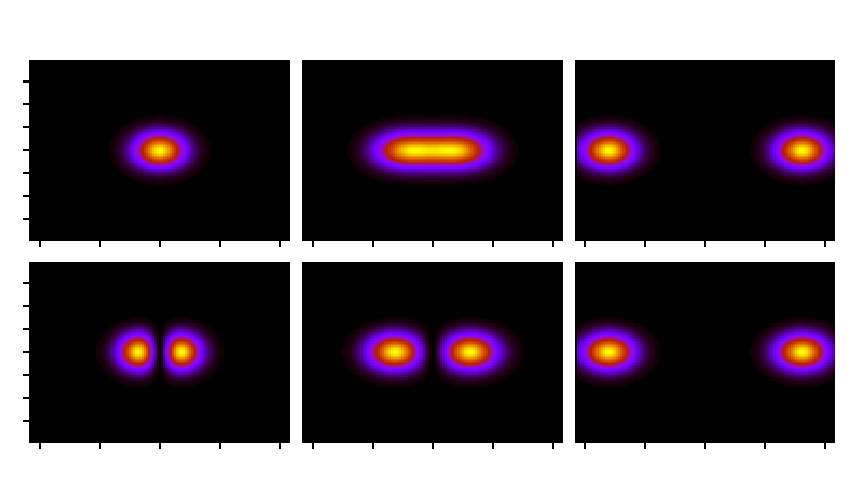
\includegraphics{images/phononProjGrdPol}}%
    \gplfronttext
  \end{picture}%
\endgroup

  \caption[Ground and first excited states projected into phonon coordinates.]
  {Projection into phonon coordinates for the ground (top) and first excited (bottom) states for three different values of the coupling parameter $\lambda_{ir}$.}
  \label{fig:phononProjGrdPol}
\end{figure}

The polaron-tunneling energy $\omega_1$, at the relevant $\lambda_{ir}=0.1263$ eV is 141.39 cm$^{-1}$, corresponding to a characteristic temperature $T=\hbar\omega_1 / k_B \sim 204$ K.
Thus the atomic motion in the cluster, in the temperature range where the pseudogap is present, can be described by a two-level Hamiltonian $\tilde{H}=(\omega_1/2)\sigma_z$,  such that $\tilde{H}\ket{\psi_1}=+(\omega_1/2)\ket{\psi_1}$ and $\tilde{H}\ket{\psi_o}=-(\omega_1/2)\ket{\psi_0}$, where $\sigma_z$ is a Pauli spin matrix and $\ket{\psi_0},\ket{\psi_1}$ denote the (symmetric) ground state and (antisymmetric) first excited state, respectively, separated by a \textit{polaron tunneling} energy $\hbar\omega_1$ \cite{MustredeLeon1990}.

% Figure of projection into definite electron-occupation basis for both, the ground and polaron-tunneling state

\section{Bipolaron binding energy}
\label{sec:PolBindingEnergy}

The energy of the ground state also changes with the coupling parameter $\lambda_{ir}$.
The change in energy between the coupled and uncoupled systems, $\Delta\omega_{g}$, can be identified, in the region where there are bipolaronic objects present, as the \textit{bipolaron binding energy}.
In figure \ref{fig:polaronFormation} we show the dependence of $\Delta\omega_{g}$ with $\lambda_{ir}$.

\begin{figure}[ht]
  \centering
  % GNUPLOT: LaTeX picture with Postscript
\begingroup
  \makeatletter
  \providecommand\color[2][]{%
    \GenericError{(gnuplot) \space\space\space\@spaces}{%
      Package color not loaded in conjunction with
      terminal option `colourtext'%
    }{See the gnuplot documentation for explanation.%
    }{Either use 'blacktext' in gnuplot or load the package
      color.sty in LaTeX.}%
    \renewcommand\color[2][]{}%
  }%
  \providecommand\includegraphics[2][]{%
    \GenericError{(gnuplot) \space\space\space\@spaces}{%
      Package graphicx or graphics not loaded%
    }{See the gnuplot documentation for explanation.%
    }{The gnuplot epslatex terminal needs graphicx.sty or graphics.sty.}%
    \renewcommand\includegraphics[2][]{}%
  }%
  \providecommand\rotatebox[2]{#2}%
  \@ifundefined{ifGPcolor}{%
    \newif\ifGPcolor
    \GPcolortrue
  }{}%
  \@ifundefined{ifGPblacktext}{%
    \newif\ifGPblacktext
    \GPblacktextfalse
  }{}%
  % define a \g@addto@macro without @ in the name:
  \let\gplgaddtomacro\g@addto@macro
  % define empty templates for all commands taking text:
  \gdef\gplbacktext{}%
  \gdef\gplfronttext{}%
  \makeatother
  \ifGPblacktext
    % no textcolor at all
    \def\colorrgb#1{}%
    \def\colorgray#1{}%
  \else
    % gray or color?
    \ifGPcolor
      \def\colorrgb#1{\color[rgb]{#1}}%
      \def\colorgray#1{\color[gray]{#1}}%
      \expandafter\def\csname LTw\endcsname{\color{white}}%
      \expandafter\def\csname LTb\endcsname{\color{black}}%
      \expandafter\def\csname LTa\endcsname{\color{black}}%
      \expandafter\def\csname LT0\endcsname{\color[rgb]{1,0,0}}%
      \expandafter\def\csname LT1\endcsname{\color[rgb]{0,1,0}}%
      \expandafter\def\csname LT2\endcsname{\color[rgb]{0,0,1}}%
      \expandafter\def\csname LT3\endcsname{\color[rgb]{1,0,1}}%
      \expandafter\def\csname LT4\endcsname{\color[rgb]{0,1,1}}%
      \expandafter\def\csname LT5\endcsname{\color[rgb]{1,1,0}}%
      \expandafter\def\csname LT6\endcsname{\color[rgb]{0,0,0}}%
      \expandafter\def\csname LT7\endcsname{\color[rgb]{1,0.3,0}}%
      \expandafter\def\csname LT8\endcsname{\color[rgb]{0.5,0.5,0.5}}%
    \else
      % gray
      \def\colorrgb#1{\color{black}}%
      \def\colorgray#1{\color[gray]{#1}}%
      \expandafter\def\csname LTw\endcsname{\color{white}}%
      \expandafter\def\csname LTb\endcsname{\color{black}}%
      \expandafter\def\csname LTa\endcsname{\color{black}}%
      \expandafter\def\csname LT0\endcsname{\color{black}}%
      \expandafter\def\csname LT1\endcsname{\color{black}}%
      \expandafter\def\csname LT2\endcsname{\color{black}}%
      \expandafter\def\csname LT3\endcsname{\color{black}}%
      \expandafter\def\csname LT4\endcsname{\color{black}}%
      \expandafter\def\csname LT5\endcsname{\color{black}}%
      \expandafter\def\csname LT6\endcsname{\color{black}}%
      \expandafter\def\csname LT7\endcsname{\color{black}}%
      \expandafter\def\csname LT8\endcsname{\color{black}}%
    \fi
  \fi
  \setlength{\unitlength}{0.0500bp}%
  \begin{picture}(6802.00,3968.00)%
    \gplgaddtomacro\gplbacktext{%
      \colorrgb{0.31,0.31,0.31}%
      \put(946,751){\makebox(0,0)[r]{\strut{}-600}}%
      \colorrgb{0.31,0.31,0.31}%
      \put(946,1235){\makebox(0,0)[r]{\strut{}-500}}%
      \colorrgb{0.31,0.31,0.31}%
      \put(946,1719){\makebox(0,0)[r]{\strut{}-400}}%
      \colorrgb{0.31,0.31,0.31}%
      \put(946,2203){\makebox(0,0)[r]{\strut{}-300}}%
      \colorrgb{0.31,0.31,0.31}%
      \put(946,2687){\makebox(0,0)[r]{\strut{}-200}}%
      \colorrgb{0.31,0.31,0.31}%
      \put(946,3171){\makebox(0,0)[r]{\strut{}-100}}%
      \colorrgb{0.31,0.31,0.31}%
      \put(946,3655){\makebox(0,0)[r]{\strut{} 0}}%
      \colorrgb{0.31,0.31,0.31}%
      \put(1125,484){\makebox(0,0){\strut{} 0}}%
      \colorrgb{0.31,0.31,0.31}%
      \put(2181,484){\makebox(0,0){\strut{} 0.05}}%
      \colorrgb{0.31,0.31,0.31}%
      \put(3237,484){\makebox(0,0){\strut{} 0.1}}%
      \colorrgb{0.31,0.31,0.31}%
      \put(4293,484){\makebox(0,0){\strut{} 0.15}}%
      \colorrgb{0.31,0.31,0.31}%
      \put(5349,484){\makebox(0,0){\strut{} 0.2}}%
      \colorrgb{0.31,0.31,0.31}%
      \put(6405,484){\makebox(0,0){\strut{} 0.25}}%
      \csname LTb\endcsname%
      \put(176,2227){\rotatebox{-270}{\makebox(0,0){\strut{}$\Delta\omega_g (meV)$}}}%
      \put(3765,154){\makebox(0,0){\strut{}$\lambda_{ir}$ (eV)}}%
      \put(3871,1105){\makebox(0,0)[l]{\strut{}\scriptsize$\lambda_{ir}=0.1263$}}%
    }%
    \gplgaddtomacro\gplfronttext{%
    }%
    \gplbacktext
    \put(0,0){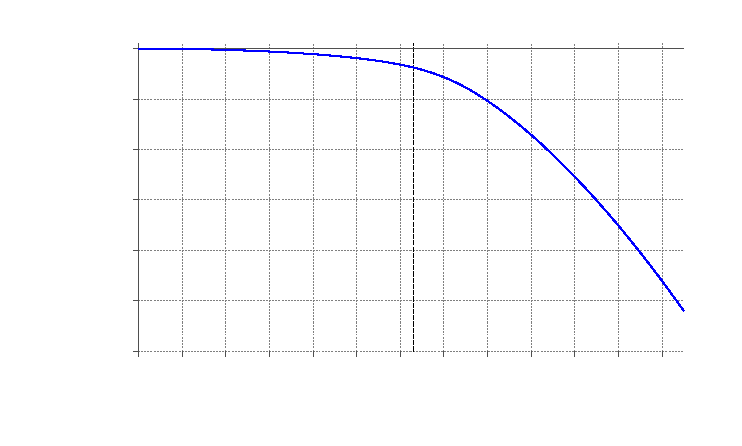
\includegraphics{images/polaronFormation}}%
    \gplfronttext
  \end{picture}%
\endgroup

  \caption[Bipolaron formation energy as a function of the $\lambda_{ir}$ coupling. ]
  {Bipolaron formation energy as a function of the $\lambda_{ir}$ coupling. The vertical line is drawn at the relevant value $\lambda_{ir}=0.1263$ eV.}
  \label{fig:polaronFormation}
\end{figure}

We observe a monotonical behaviour with a small change in the weak coupling regime becoming stronger with greater coupling values.
In particular, for the $\lambda_{ir}=0.1263$ eV value, which reproduces the observed distortion, we find $\Delta\omega_{g} \sim 38$ meV.
This value compares favorably with the value obtained from femtosecond time-domain spectroscopy ($\sim 45$ meV) for YBa$_2$Cu$_3$O$_7$ \cite{Demsar1999}. 
We also find that if we consider a smaller electron-lattice coupling such that the distortion is 0.08 \AA\ ($\lambda_{ir}=0.124$ eV), as that observed for in plane Cu(2)-O in La$_{1.85}$Sr$_{0.15}$CuO$_4$ \cite{Bianconi1996}, we obtain $\Delta\omega_{g} \sim 35$ meV, which is also comparable to estimates for the pseudogap formation energy in this system (see Fig. 4b in \cite{Kusar2005}).

Furthermore, we calculated the isotopic shift, $\Delta_g$, of $\omega_g$ under the $^{16}$O$\rightarrow ^{18}$O substitution as defined in (\ref{eq:isot-shift-def-grd}).
Figure \ref{fig:isotPolaronFormation} shows $\Delta_g$ as a function of $\lambda_{ir}$.
Contrary to other isotopic shifts, it does not change sign.
However, it shows a maximum in the middle coupling regime, reminiscent of the maxima, minima and inflection points in the isotopic shifts of all other excitations, and falls below its starting point for large $\lambda_{ir}$ values.
For $\lambda_{ir}=0.1263$ eV we predict an isotopic shift of $\sim 9.2$ \% which is slightly larger than the uncoupled value of $\sim 7.2$ \%.

\begin{figure}[ht]
  \centering
  % GNUPLOT: LaTeX picture with Postscript
\begingroup
  \makeatletter
  \providecommand\color[2][]{%
    \GenericError{(gnuplot) \space\space\space\@spaces}{%
      Package color not loaded in conjunction with
      terminal option `colourtext'%
    }{See the gnuplot documentation for explanation.%
    }{Either use 'blacktext' in gnuplot or load the package
      color.sty in LaTeX.}%
    \renewcommand\color[2][]{}%
  }%
  \providecommand\includegraphics[2][]{%
    \GenericError{(gnuplot) \space\space\space\@spaces}{%
      Package graphicx or graphics not loaded%
    }{See the gnuplot documentation for explanation.%
    }{The gnuplot epslatex terminal needs graphicx.sty or graphics.sty.}%
    \renewcommand\includegraphics[2][]{}%
  }%
  \providecommand\rotatebox[2]{#2}%
  \@ifundefined{ifGPcolor}{%
    \newif\ifGPcolor
    \GPcolortrue
  }{}%
  \@ifundefined{ifGPblacktext}{%
    \newif\ifGPblacktext
    \GPblacktextfalse
  }{}%
  % define a \g@addto@macro without @ in the name:
  \let\gplgaddtomacro\g@addto@macro
  % define empty templates for all commands taking text:
  \gdef\gplbacktext{}%
  \gdef\gplfronttext{}%
  \makeatother
  \ifGPblacktext
    % no textcolor at all
    \def\colorrgb#1{}%
    \def\colorgray#1{}%
  \else
    % gray or color?
    \ifGPcolor
      \def\colorrgb#1{\color[rgb]{#1}}%
      \def\colorgray#1{\color[gray]{#1}}%
      \expandafter\def\csname LTw\endcsname{\color{white}}%
      \expandafter\def\csname LTb\endcsname{\color{black}}%
      \expandafter\def\csname LTa\endcsname{\color{black}}%
      \expandafter\def\csname LT0\endcsname{\color[rgb]{1,0,0}}%
      \expandafter\def\csname LT1\endcsname{\color[rgb]{0,1,0}}%
      \expandafter\def\csname LT2\endcsname{\color[rgb]{0,0,1}}%
      \expandafter\def\csname LT3\endcsname{\color[rgb]{1,0,1}}%
      \expandafter\def\csname LT4\endcsname{\color[rgb]{0,1,1}}%
      \expandafter\def\csname LT5\endcsname{\color[rgb]{1,1,0}}%
      \expandafter\def\csname LT6\endcsname{\color[rgb]{0,0,0}}%
      \expandafter\def\csname LT7\endcsname{\color[rgb]{1,0.3,0}}%
      \expandafter\def\csname LT8\endcsname{\color[rgb]{0.5,0.5,0.5}}%
    \else
      % gray
      \def\colorrgb#1{\color{black}}%
      \def\colorgray#1{\color[gray]{#1}}%
      \expandafter\def\csname LTw\endcsname{\color{white}}%
      \expandafter\def\csname LTb\endcsname{\color{black}}%
      \expandafter\def\csname LTa\endcsname{\color{black}}%
      \expandafter\def\csname LT0\endcsname{\color{black}}%
      \expandafter\def\csname LT1\endcsname{\color{black}}%
      \expandafter\def\csname LT2\endcsname{\color{black}}%
      \expandafter\def\csname LT3\endcsname{\color{black}}%
      \expandafter\def\csname LT4\endcsname{\color{black}}%
      \expandafter\def\csname LT5\endcsname{\color{black}}%
      \expandafter\def\csname LT6\endcsname{\color{black}}%
      \expandafter\def\csname LT7\endcsname{\color{black}}%
      \expandafter\def\csname LT8\endcsname{\color{black}}%
    \fi
  \fi
  \setlength{\unitlength}{0.0500bp}%
  \begin{picture}(6802.00,3968.00)%
    \gplgaddtomacro\gplbacktext{%
      \colorrgb{0.31,0.31,0.31}%
      \put(726,751){\makebox(0,0)[r]{\strut{}\scriptsize 5}}%
      \colorrgb{0.31,0.31,0.31}%
      \put(726,1243){\makebox(0,0)[r]{\strut{}\scriptsize 6}}%
      \colorrgb{0.31,0.31,0.31}%
      \put(726,1735){\makebox(0,0)[r]{\strut{}\scriptsize 7}}%
      \colorrgb{0.31,0.31,0.31}%
      \put(726,2227){\makebox(0,0)[r]{\strut{}\scriptsize 8}}%
      \colorrgb{0.31,0.31,0.31}%
      \put(726,2719){\makebox(0,0)[r]{\strut{}\scriptsize 9}}%
      \colorrgb{0.31,0.31,0.31}%
      \put(726,3211){\makebox(0,0)[r]{\strut{}\scriptsize 10}}%
      \colorrgb{0.31,0.31,0.31}%
      \put(726,3703){\makebox(0,0)[r]{\strut{}\scriptsize 11}}%
      \colorrgb{0.31,0.31,0.31}%
      \put(905,484){\makebox(0,0){\strut{}\scriptsize 0}}%
      \colorrgb{0.31,0.31,0.31}%
      \put(2005,484){\makebox(0,0){\strut{}\scriptsize 0.05}}%
      \colorrgb{0.31,0.31,0.31}%
      \put(3105,484){\makebox(0,0){\strut{}\scriptsize 0.1}}%
      \colorrgb{0.31,0.31,0.31}%
      \put(4205,484){\makebox(0,0){\strut{}\scriptsize 0.15}}%
      \colorrgb{0.31,0.31,0.31}%
      \put(5305,484){\makebox(0,0){\strut{}\scriptsize 0.2}}%
      \colorrgb{0.31,0.31,0.31}%
      \put(6405,484){\makebox(0,0){\strut{}\scriptsize 0.25}}%
      \csname LTb\endcsname%
      \put(352,2227){\rotatebox{-270}{\makebox(0,0){\strut{}$\Delta_g\ (meV)$}}}%
      \put(3655,154){\makebox(0,0){\strut{}$\lambda_{ir}$ (eV)}}%
      \put(3765,1105){\makebox(0,0)[l]{\strut{}\scriptsize$\lambda_{ir}=0.1263$}}%
    }%
    \gplgaddtomacro\gplfronttext{%
    }%
    \gplbacktext
    \put(0,0){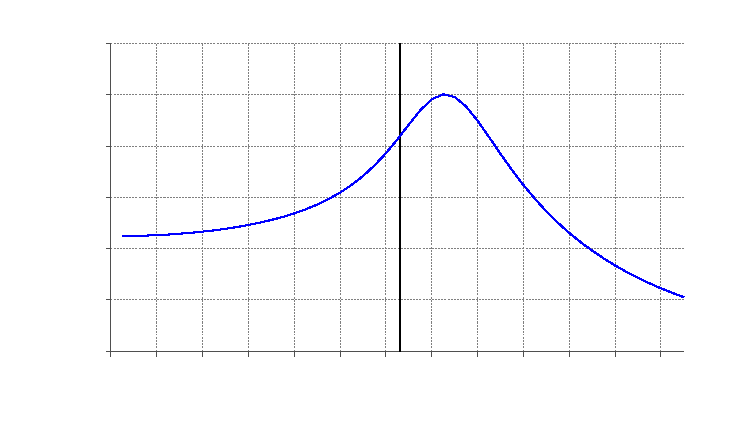
\includegraphics{images/isotPolaronFormation}}%
    \gplfronttext
  \end{picture}%
\endgroup

  \caption[Isotopic shift of the bipolaron formation energy.]
  {Isotopic shift of the bipolaron formation energy. The vertical line is placed at the relevant value $\lambda_{ir}=0.1263$.}
  \label{fig:isotPolaronFormation}
\end{figure}



